\documentclass[12pt,a4paper,final]{article}

\usepackage[utf8]{inputenc}
\usepackage[T1]{fontenc}
\usepackage[french]{babel}
\usepackage{graphicx}
\usepackage{float}
\usepackage{hyperref}
\usepackage{placeins}

\title{Hacker votre adaptateur ADB/USB}
\author{Jean THOMAS}
\date{}

\begin{document}

\maketitle

\section{Introduction}

L'adaptateur ADB/USB utilise le firmware open source tmk\_keyboard. Il est donc possible de bidouiller de le firmware de votre adaptateur pour changer le mapping du clavier pour l'adapter à votre utilisation. Nous verrons dans ce guide comment flasher un nouveau firmware sur votre adaptateur ADB/USB, et comment modifier le firmware tmk\_keyboard pour adapter le mapping du clavier à votre convenance.

Il est important de noter que ce document ne s'adresse qu'aux utilisateurs de la révision 0x1. La révision de votre adaptateur est indiquée au dos du circuit imprimé.

\section{Flasher l'adaptateur}

\subsection{Le connecteur ISP}

Le connecteur ISP est un connecteur qui permet de programmer un micro-contrôleur sans devoir l'extraire physiquement. Sur votre convertisseur, le connecteur ISP se situe à droite du connecteur ADB.

\begin{figure}[h]
    \centering
    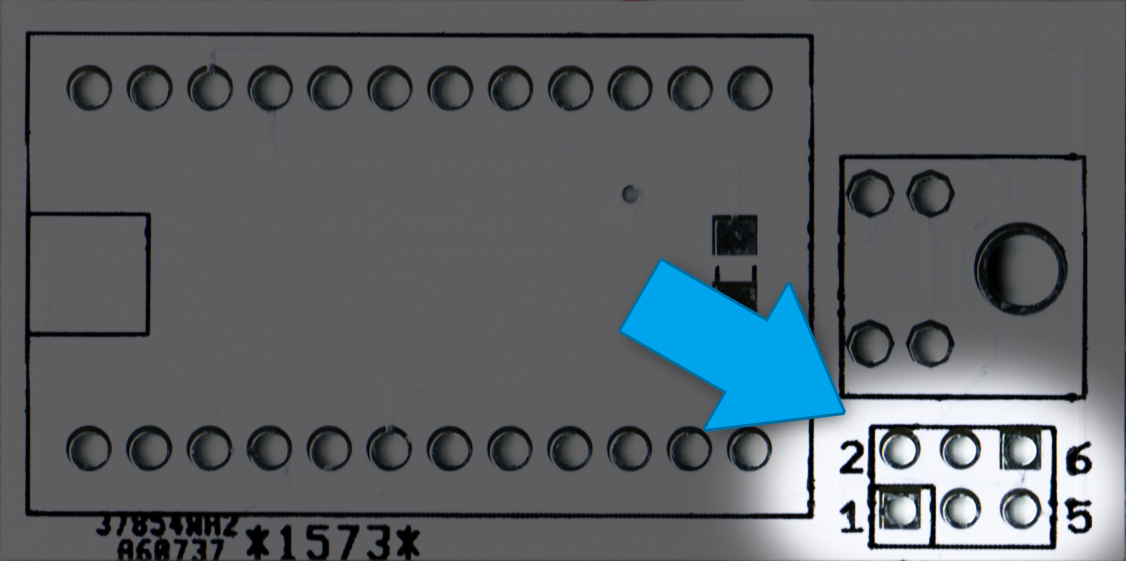
\includegraphics[width=6cm]{isp_connector.jpg}
    \caption{Le connecteur ISP sur le circuit imprimé}
    \label{fig:1}
\end{figure}

\FloatBarrier

Pour pouvoir l'utiliser, il faut souder un connecteur male type HE14. Ce connecteur se trouve à bas prix en magasin d'électronique. Vous pouvez utiliser au choix deux connecteurs 3 broches simple rangée, côte à côte, ou alors utiliser un connecteur double rangée de 6 broches.

\subsection{Le programmateur AVR}

Un programmateur AVR est un dispositif qui joue le rôle d'interface entre notre ordinateur et notre convertisseur ADB/USB, pour pouvoir programmer ce dernier. Il existe plusieurs types de programmateurs AVR. Dans ce guide je traiterai du programmateur USBasp. Il est économique, simple à utiliser, et surtout compatible avec Mac OS X.

\begin{figure}[h]
    \centering
    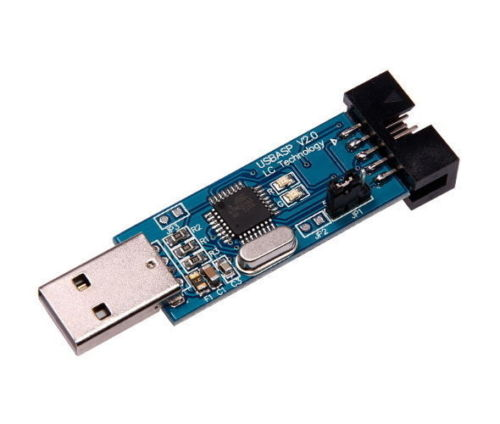
\includegraphics[width=6cm]{usbasp.jpg}
    \caption{Le programmateur USBasp}
    \label{fig:2}
\end{figure}

\FloatBarrier

Ce programmateur est doté d'un connecteur ISP 10 broches. Pour des raisons de place, il n'est pas possible d'en intégrer un sur les convertisseurs ADB/USB. Nous utiliserons alors un adaptateur passif ISP 10 broches vers ISP 6 broches, qui peut être fabriqué facilement si on dispose des connecteurs adéquats, ou sinon peut être acheté à très bas prix.

\begin{figure}[h]
    \centering
    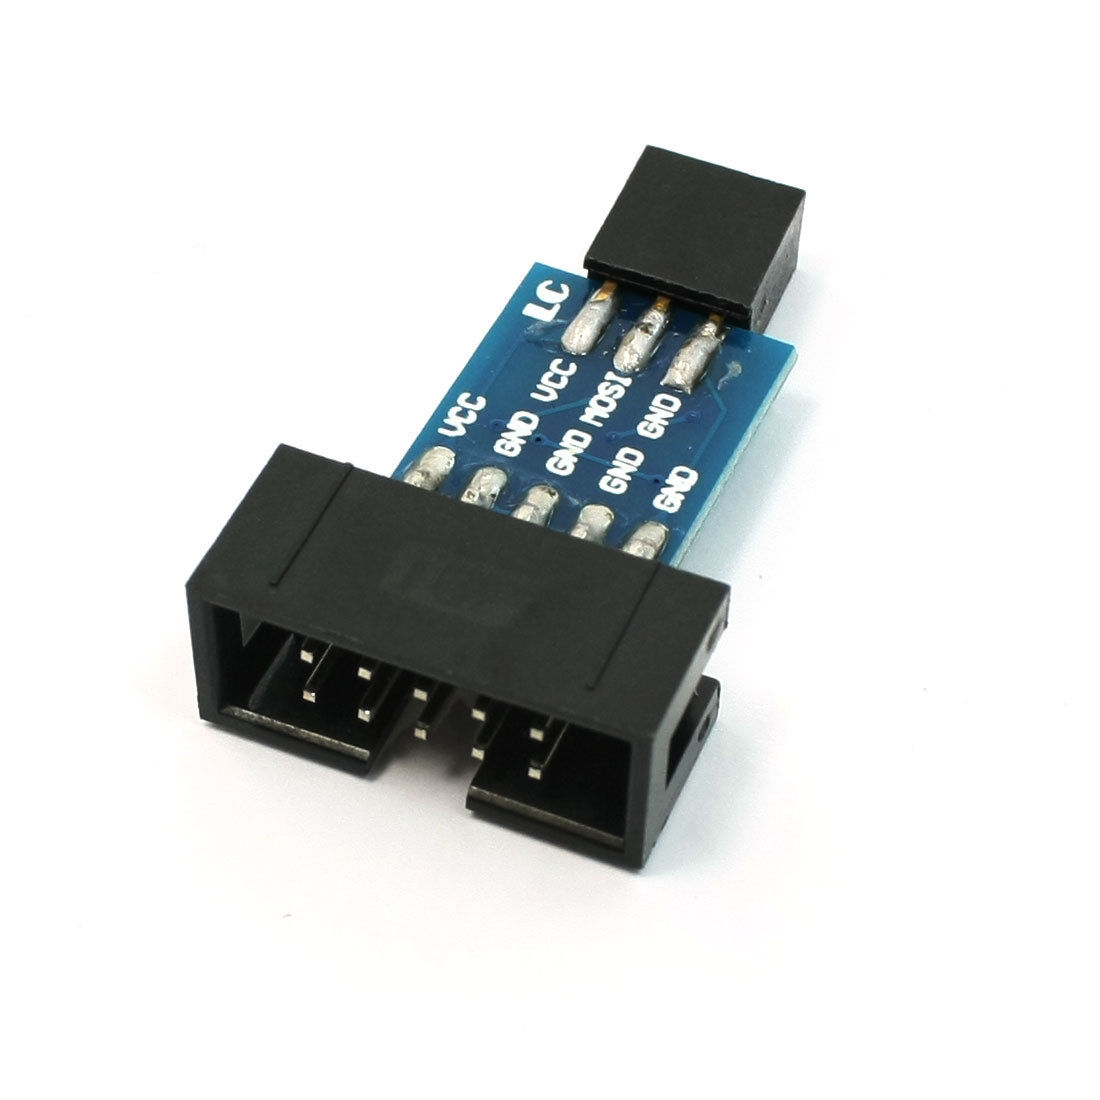
\includegraphics[width=4cm]{isp_adapter.jpg}
    \caption{L'adaptateur ISP 10 broches vers 6 broches}
    \label{fig:3}
\end{figure}

\FloatBarrier

N'oubliez pas de respecter le sens de branchement sur le côté ISP 6 broches (l'autre côté étant doté d'un détrompeur) : la patte GND de l'adaptateur correspond à la broche 6 de l'adaptateur ADB/USB.

\subsection{avrdude}

Pour utiliser le programmateur sous Mac OS X, nous allons utiliser un logiciel nommé "avrdude", qui peut être installé grâce à homebrew (\url{http://brew.sh}).

On l'installe à l'aide d'une simple commande dans le terminal :

\begin{verbatim}
brew install avrdude
\end{verbatim}

Une fois avrdude installé, nous pouvons l'utiliser pour flasher le firmware sur l'adaptateur :

\begin{verbatim}
avrdude -c usbasp -p m32u4 -U flash:w:monfirmware.hex
\end{verbatim}

Ici, le firmware flashé est nommé \textbf{monfirmware.hex}.

\section{Compiler tmk\_keyboard}

\subsection{Installer le toolchain}

Pour compiler le firmware, nous allons avoir besoin de deux outils : Git, qui nous servira à récupérer le firmware, et le toolchain, qui est l'ensemble des outils nécessaires à la compilation.
L'installation se fait automatiquement dans le terminal grâce à homebrew, en tapant deux commandes à la suite :

\begin{verbatim}
brew tap larsimmisch/avr
brew install avr-libc git
\end{verbatim}

\subsection{Récupérer le firmware}

Le firmware tmk\_keyboard est hébergé sur Github, pour le télécharger nous allons utiliser Git dans le terminal :

\begin{verbatim}
git clone https://github.com/tmk/tmk_keyboard
\end{verbatim}

Ensuite il faut se déplacer jusqu'au dossier contenant les sources du firmware du convertisseur ADB/USB :

\begin{verbatim}
cd tmk_keyboard/converter/adb_usb/
\end{verbatim}

\subsection{La compilation}

La compilation s'effectue avec la commande \textbf{make} :

\begin{verbatim}
make KEYMAP=iso
\end{verbatim}

Je précise \textbf{KEYMAP=iso} car l'adaptateur est adapté aux claviers européens. Si vous ne précisez pas le mapping au Makefile, le firmware sera adapté pour les claviers ANSI (américains).
Vous aurez alors un fichier nommé \textbf{adb\_usb\_lufa.hex}, qui contiendra le firmware compilé. Vous pouvez à présent le flasher à l'aide d'avrdude :

\begin{verbatim}
avrdude -c usbasp -p m32u4 -U flash:w:adb_usb_lufa.hex
\end{verbatim}

\subsection{Modifier l'agencement des touches}

Pour modifier l'agencement des touches, nous allons devoir toucher au code source de tmk\_keyboard, en particulier au fichier \textbf{keymap\_iso.c} (situé dans \textbf{/tmk\_keyboard/converter/adb\_usb/}) qui contient le mapping du clavier en ISO.

\begin{figure}[h]
    \centering
    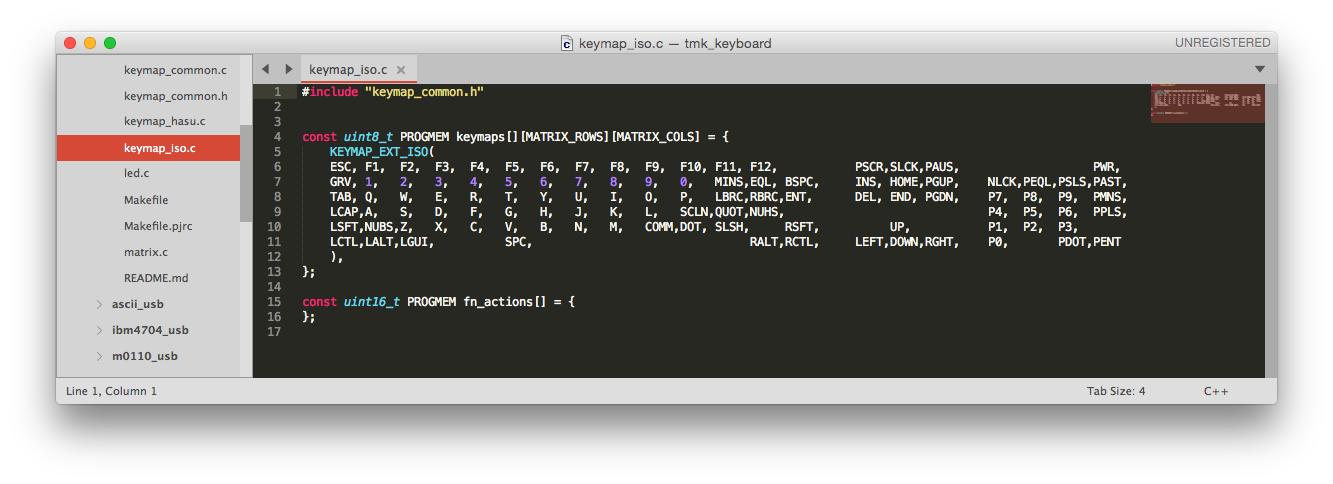
\includegraphics[width=14cm]{keymap_iso.png}
    \caption{Le fichier keymap\_iso.c par défaut}
    \label{fig:4}
\end{figure}

\FloatBarrier

Chaque touche physique du clavier est assignée à un code (par exemple \textbf{LCTL} pour la touche contrôle gauche). Il est possible de modifier le code d'une touche, pour lui assigner une autre fonctionnalité.

Par exemple, si je veux assigner la touche shift droite à la fonction espace, je devrai remplacer \textbf{RSFT} par \textbf{SPC}.

Il me suffira ensuite de re-compiler le firmware à l'aide des instructions ci-dessus, et de flasher mon firmware personnalisé.
\\[12pt]

Il existe quelques codes intéressants, par exemple ceux des touches multimédias :

\begin{verbatim}
AUDIO_MUTE : coupe le son
AUDIO_VOL_UP : augmente le volume
AUDIO_VOL_DOWN : baisse le volume
MEDIA_NEXT_TRACK : joue le média suivante
MEDIA_PREV_TRACK : joue le média précédent
MEDIA_STOP : arrête toute lecture de média
MEDIA_PLAY_PAUSE : met en pause le média
MEDIA_EJECT : éjection
\end{verbatim}

Une liste détaillée de tous les codes intéressants se trouve dans le fichier \textbf{keycode.h} (situé dans \textbf{/tmk\_keyboard/common/}). N'oubliez pas d'enlever le préfixe \textbf{KC\_} pour utiliser le code de touche dans votre \textbf{keymap\_iso.c} !

\end{document}